
\section{Antecedentes}
Puchleitner et al. \cite{Puchleitner2026} abordaron la problemática de la ineficiencia y la alta demanda de tiempo que caracteriza a la Ingeniería de 
Requisitos (IR), proceso crítico cuyo manejo deficiente suele comprometer sistemáticamente el éxito de los proyectos de software. El estudio tuvo como 
objetivo evaluar el desempeño de los modelos de lenguaje de gran tamaño (LLM) en la generación de especificaciones funcionales coherentes y 
contextualmente relevantes a partir del alcance de un proyecto. Para ello, se aplicó una metodología comparativa analítica utilizando los modelos 
GPT-4o y Llama-3-70b-instruct sobre tres proyectos del dataset PURE, empleando una estructura de prompt refinada que definía roles especializados y 
priorizaba las salidas por nivel de importancia. Los resultados revelaron que aproximadamente el 80\% de los requisitos generados por ambos modelos 
poseían relevancia funcional, logrando un solapamiento de contenido superior al 88\% en aquellos clasificados con mayor prioridad. Asimismo, el análisis 
crítico detectó que las divergencias semánticas y la inclusión de requisitos implícitos representan los principales desafíos para alcanzar una alineación 
total con las especificaciones humanas. Este trabajo sustenta la presente investigación al validar empíricamente que la IA generativa puede automatizar 
tareas de documentación técnica inicial con alta precisión, sentando un precedente fundamental para el desarrollo de sistemas que busquen optimizar la 
fase de especificación mediante el uso de arquitecturas inteligentes \cite{Puchleitner2026}.


Sami et al. \cite{Sami2026} abordaron la ineficiencia y falta de consistencia inherente a la especificación y priorización manual de historias de
usuario en marcos de trabajo ágiles. El estudio tuvo como propósito evaluar la eficacia de un sistema multi-agente basado en roles, implementando 
modelos de lenguaje de gran tamaño (LLM) como GPT-4o y Llama 3.3 para automatizar estos procesos críticos. La metodología consistió en simular la 
interacción de un equipo de desarrollo conformado por agentes especialistas (Dueño del Producto, Desarrollador y QA), quienes emplearon la técnica 
de los 100 dólares para clasificar los requisitos generados a partir de la visión de un proyecto logístico real \cite{Sami2026}. Los resultados 
evidenciaron que, si bien todos los modelos producen requisitos con alta relevancia funcional y similitud semántica, GPT-4o demostró una cobertura 
más exhaustiva de las fases del proyecto en comparación con sus pares \cite{Sami2026}. Asimismo, el análisis crítico reveló que la alineación con el 
juicio experto humano es moderada, enfrentando dificultades para capturar contextos de dominio dinámicos y matizados \cite{Sami2026}. Por otra parte, 
se concluyó que la variabilidad entre ejecuciones persiste como un desafío técnico para la estabilidad de las propuestas generadas. Esta investigación 
sustenta la presente tesis al validar el potencial de las arquitecturas multi-agente para orquestar perspectivas técnicas diversas en la Ingeniería de 
Requisitos, subrayando a la vez la necesidad de refinar los mecanismos de integración de contexto para alcanzar una autonomía superior en la documentación 
SRS \cite{Sami2026}.


Terragni et al. \cite{Terragni2025} analizan la transición hacia una ingeniería de software potenciada por IA, enfrentando el desafío de gestionar 
la creciente complejidad de los sistemas mediante niveles superiores de abstracción. El estudio tiene como objetivo proponer un marco conceptual para 
una colaboración simbiótica entre desarrolladores y sistemas multi-agente que optimice fases críticas como la ingeniería de requisitos. Mediante una 
metodología prospectiva basada en el análisis de herramientas "agentic" actuales, los autores describen una arquitectura donde agentes especializados, 
coordinados por un orquestador, ejecutan tareas de elicitación, validación y resumen de especificaciones funcionales. Los resultados sugieren que la 
evolución tecnológica conduce inevitablemente hacia sistemas autónomos capaces de percibir y actuar en el entorno de desarrollo, aunque se concluye 
que la supervisión humana es vital para garantizar la confiabilidad frente a las alucinaciones del modelo \cite{Terragni2025}. Asimismo, este trabajo 
fundamenta la presente tesis al proporcionar una base arquitectónica robusta que justifica el uso de agentes orquestados para la generación y 
verificación automática de documentación SRS profesional \cite{Terragni2025}.

Nguyen-Duc et al. \cite{Nguyen-Duc2025} abordan la carencia de una visión integral sobre los desafíos y aplicaciones prácticas de la Inteligencia 
Artificial Generativa (GenAI) en la Ingeniería de Software. El estudio se propuso definir una agenda de investigación mediante una metodología que 
integró una revisión de literatura con cuatro grupos focales de expertos durante un periodo de cinco meses. Entre los resultados principales, se 
identificaron 78 preguntas de investigación abiertas, subrayando que áreas críticas como la ingeniería de requisitos han recibido menor atención frente 
a la implementación de código, enfrentando obstáculos como alucinaciones, sesgos y limitaciones en el procesamiento de contexto 
global \cite{Nguyen-Duc2025}. Asimismo, los autores resaltan la visión de utilizar agentes de IA basados en roles para la automatización 
de proyectos, lo cual guarda una relación directa con esta investigación al fundamentar la transición hacia arquitecturas multi-agente. Por 
otra parte, el estudio concluye que el futuro de la disciplina radica en plataformas de colaboración simbiótica humano-IA, sustentando la pertinencia 
de automatizar la generación de requisitos para optimizar la productividad y la calidad documental \cite{Nguyen-Duc2025}.

Mahbub et al. \cite{Mahbub2024} abordaron la problemática de los defectos en especificaciones de requisitos de software (SRS) industriales, cuya 
detección manual resulta ineficiente en documentos extensos y complejos. El objetivo del estudio fue evaluar el desempeño de GPT-4, bajo un enfoque 
de aprendizaje de disparo cero (zero-shot), en la identificación de ambigüedades, inconsistencias e incompletitud dentro de un SRS de 52 páginas para 
un sistema de ventilación mecánica. La metodología empleada incluyó el procesamiento de segmentos textuales y descripciones de diagramas UML, permitiendo 
comparar los hallazgos de la IA con el criterio de expertos humanos. Los resultados destacaron una precisión de 0.61 para detectar omisiones, aunque el 
rendimiento decreció significativamente en inconsistencias (0.43) y ambigüedades (0.39) \cite{Mahbub2024}. El análisis concluyó que, si bien la IA 
facilita una detección temprana y recupera el 60\% de los fallos identificados por especialistas, presenta limitaciones críticas en la gestión del 
contexto global y el conocimiento de dominio profundo \cite{Mahbub2024}. Asimismo, esta investigación es fundamental para la presente tesis, ya que 
evidencia la necesidad de implementar mecanismos de validación automática que superen las restricciones de contexto detectadas mediante arquitecturas 
más sofisticadas.


Binkhonain y Alfayaz \cite{Binkhonain2025} abordan la problemática de la dependencia de grandes conjuntos de datos etiquetados y la escasa capacidad 
de generalización de los modelos supervisados tradicionales en la clasificación de requisitos de software. El objetivo del estudio fue evaluar la 
efectividad de los modelos de lenguaje de gran tamaño (LLM) y diversas técnicas de prompting para automatizar esta tarea crítica. La metodología 
consistió en un estudio de referencia empírico que comparó cinco modelos, tales como GPT-4 Turbo y Gemini 2.0 Flash, aplicando estrategias de zero-shot, 
few-shot, persona y cadena de pensamiento sobre los datasets PROMISE y SecReq. Los resultados evidenciaron que la configuración few-shot, potenciada con 
la asignación de roles, logra un rendimiento superior o comparable al de modelos especializados como BERT \cite{Binkhonain2025}. Asimismo, se concluyó 
que el uso de LLMs basados en instrucciones ofrece una solución flexible y escalable que minimiza la necesidad de reentrenamiento manual. Por otra parte, 
este trabajo sustenta la presente tesis al validar técnicamente el uso de IA generativa para el tratamiento de requisitos, demostrando que la 
especialización instruccional es un pilar fundamental para la automatización de la documentación funcional y técnica \cite{Binkhonain2025}.


Maestre Peña et al. \cite{Pea2026} abordan la ineficiencia en el procesamiento del masivo volumen de retroalimentación de usuarios en plataformas 
digitales para la Ingeniería de Requisitos. El objetivo del estudio fue desarrollar un método híbrido que integra modelos de Aprendizaje Profundo 
para el filtrado de datos y Modelos de Lenguaje de Gran Tamaño (LLM) para la especificación automática de requisitos. La metodología implementada 
consistió en tres fases: clasificación de opiniones informativas mediante BERTweet con inyección de conocimiento técnico (ISO/IEC/IEEE 24765), 
agrupamiento temático basado en Fuzzy C-Means y generación mediante DeepSeek V3 utilizando un prompt estructurado por etapas. Los resultados obtenidos 
en cuatro conjuntos de datos reales evidenciaron un rendimiento superior a soluciones estatales, logrando un F1-Score promedio de 0.950 y garantizando 
la trazabilidad hacia la fuente original \cite{Pea2026}. Asimismo, el estudio concluye que la calidad de la documentación generada depende críticamente 
de la organización y el filtrado previo de la información contextual. Por otra parte, este antecedente es fundamental para la presente investigación, 
ya que valida la efectividad de los LLM en la transformación de lenguaje natural informal en especificaciones funcionales bajo criterios de calidad, 
sentando las bases técnicas para el uso de arquitecturas inteligentes en la automatización de la documentación SRS \cite{Pea2026}.


Aboukadri et al. \cite{Aboukadri2025} abordan la problemática de la ineficiencia y los errores inherentes a la identificación manual de políticas de 
control de acceso en entornos ágiles, donde la seguridad suele ser relegada. El objetivo de su estudio fue automatizar la extracción y organización de 
estas políticas a partir de historias de usuario mediante un marco de trabajo que integra Generación Aumentada por Recuperación (RAG) y Modelos de 
Lenguaje de Gran Tamaño (LLM). La metodología empleada consistió en un pipeline de procesamiento que utiliza el modelo "all-distilroberta-v1" para 
generar representaciones vectoriales y almacenar fragmentos de texto en bases de datos semánticas para su posterior recuperación contextual. Pruebas 
realizadas sobre 22 conjuntos de datos con más de 1,600 historias de usuario demostraron precisiones de hasta el 84.21\%, evidenciando la capacidad de 
la IA para capturar reglas de acceso complejas de manera escalable \cite{Aboukadri2025}. Asimismo, el estudio concluye que el uso de RAG mitiga las 
alucinaciones y proporciona trazabilidad, aunque reconoce una dependencia crítica de la calidad del texto de entrada. Por otra parte, este antecedente 
sustenta la presente tesis al validar técnicamente el uso de agentes inteligentes y técnicas de recuperación de contexto para transformar requisitos 
informales en especificaciones funcionales estructuradas \cite{Aboukadri2025}.


Zhang et al. \cite{Zhang2024} abordaron la problemática de la inconsistencia y la ambigüedad en la redacción de historias de usuario, factores que 
comprometen la velocidad del desarrollo y el cumplimiento de las expectativas del cliente en marcos ágiles. El estudio se propuso evaluar la viabilidad 
de un sistema de agentes autónomos basado en modelos de lenguaje de gran tamaño (LLM), denominado ALAS, para automatizar la mejora de la calidad de estos 
requisitos funcionales. La metodología implementada consistió en una arquitectura multi-agente donde perfiles simulados de dueño de producto (PO) e 
ingeniero de requisitos (RE) interactúan de forma iterativa para refinar descripciones y criterios de aceptación bajo el marco INVEST. Pruebas realizadas 
en la organización Austrian Post Group IT utilizando modelos GPT-3.5 y GPT-4 revelaron que la intervención de la IA mejora notablemente la claridad y 
la especificidad del valor de negocio, aunque se observó que modelos más avanzados como GPT-4 tienden a producir requisitos excesivamente largos y 
complejos \cite{Zhang2024}. Asimismo, el análisis crítico concluyó que la supervisión humana sigue siendo indispensable para monitorear la integridad 
de los resultados y mitigar posibles alucinaciones. Por otra parte, esta investigación sustenta la presente tesis al validar empíricamente que la 
colaboración entre agentes especializados es una estrategia eficaz para la transformación y el refinamiento automático de especificaciones funcionales 
bajo estándares de calidad industrial \cite{Zhang2024}.

Hou et al. \cite{hou2025model} abordaron la problemática de la fragmentación tecnológica en la integración de herramientas de inteligencia artificial, la cual 
genera sistemas rígidos y difíciles de escalar debido a la dependencia de conexiones manuales de APIs. El objetivo central del estudio fue sistematizar 
el análisis del Model Context Protocol (MCP) para evaluar su arquitectura, ciclo de vida y los riesgos de seguridad emergentes en entornos de agentes 
autónomos \cite{hou2025model}. La metodología empleada consistió en la formalización de dieciséis actividades clave del protocolo y la validación empírica 
de amenazas mediante el desarrollo de servidores de prueba de concepto en entornos aislados \cite{hou2025model}. Los resultados principales revelaron que el 
MCP logra unificar la comunicación bidireccional y el descubrimiento dinámico de recursos, aunque expone vulnerabilidades críticas como la inyección 
indirecta de instrucciones y el envenenamiento de herramientas \cite{hou2025model}. Asimismo, se concluye que la madurez de este ecosistema requiere protocolos 
de validación de identidad y mecanismos de aislamiento más estrictos para garantizar la integridad de las operaciones \cite{hou2025model}. De igual manera, 
este trabajo sustenta la presente investigación al proporcionar la base técnica del protocolo MCP, facilitando que una arquitectura multi-agente recupere 
contextos externos de forma estandarizada para la generación automática de requisitos funcionales de alta precisión \cite{hou2025model}.



\section{Ingeniería de Requisitos }
La Ingeniería de Requisitos es una disciplina de la Ingeniería de Software encargada de identificar, analizar, 
documentar, validar y gestionar las necesidades y restricciones que debe satisfacer un sistema software. Su objetivo principal es asegurar
que las expectativas de los interesados sean comprendidas y representadas de manera clara, completa y verificable antes de iniciar 
las etapas de diseño e implementación \cite{Wolf2026}.

En los últimos años, el interés por automatizar algunas de estas tareas mediante técnicas de procesamiento del lenguaje natural e inteligencia
artificial ha incrementado considerablemente, debido a la necesidad de mejorar la calidad de las especificaciones y disminuir el esfuerzo asociado 
a su elaboración manual \cite{cheng2026generative}.

\subsection{Metodología de Elicitación de Requisitos}

La elicitación de requisitos es una de las actividades fundamentales de la Ingeniería de Requisitos, cuyo propósito es identificar, comprender 
y recopilar las necesidades, expectativas y restricciones de los interesados para definir las funcionalidades y características que deberá 
satisfacer el sistema software. Una adecuada ejecución de este proceso contribuye a disminuir errores derivados de requisitos incompletos, 
ambiguos o inconsistentes, reduciendo el riesgo de retrabajos y fallos durante las etapas posteriores del desarrollo \cite{Akhtar2025}, \cite{Umar2024}.

El proceso de elicitación generalmente inicia con la identificación de los interesados y continúa con la selección de técnicas apropiadas para obtener 
información del dominio del problema. Entre las técnicas más empleadas se encuentran las entrevistas, cuestionarios, talleres colaborativos, observación 
directa, análisis documental y prototipado. La elección de una técnica específica depende de factores como la complejidad del sistema, la disponibilidad 
de los participantes y el contexto organizacional en el que se desarrolla el proyecto \cite{Akhtar2025}, \cite{canedo2022guidelines}. En metodologías ágiles, la elicitación se considera una 
actividad iterativa que permite refinar continuamente los requisitos conforme evolucionan las necesidades del negocio.

En los últimos años, la incorporación de técnicas de inteligencia artificial y procesamiento del lenguaje natural ha permitido asistir el proceso 
de elicitación mediante la extracción automática de información, la identificación de requisitos implícitos y el análisis de conversaciones sostenidas 
con los interesados. Estas tecnologías buscan complementar las prácticas tradicionales y mejorar la eficiencia en la generación de especificaciones de 
requisitos, manteniendo la participación humana como elemento esencial para validar la información obtenida y garantizar su correspondencia con las 
necesidades reales de los usuarios \cite{Umar2024}.

\subsection{Estándar IEEE 830-1998}

El estándar IEEE 830-1998 establece una práctica recomendada para la elaboración de documentos de Especificación de Requisitos de Software (SRS), 
proporcionando una estructura organizada para describir de manera clara, completa y verificable las funcionalidades, restricciones y características 
de un sistema software. Entre los atributos de calidad que deben cumplir los requisitos especificados se encuentran la ausencia de ambigüedad, 
consistencia, completitud, trazabilidad y verificabilidad, con el propósito de facilitar la comunicación entre clientes, usuarios y desarrolladores 
durante el ciclo de vida del proyecto \cite{Umar2024}, \cite{Wolf2026}.

Aunque el estándar fue reemplazado posteriormente por la norma ISO/IEC/IEEE 29148, el IEEE 830-1998 continúa siendo ampliamente utilizado en entornos 
académicos y de investigación debido a la simplicidad de su estructura y a su adopción en numerosos trabajos relacionados con la automatización 
de documentos SRS. La especificación propuesta por este estándar se organiza en secciones que incluyen la introducción, descripción general del 
sistema, requisitos específicos, interfaces externas, requisitos funcionales, restricciones de diseño y otros atributos de calidad relevantes para 
el sistema desarrollado \cite{Akhtar2025}.

Si bien la norma ISO/IEC/IEEE 29148 ha sustituido oficialmente al IEEE 830-1998, este último sigue teniendo vigencia en el ámbito académico. 
Su estructura clara y su extensa utilización en estudios enfocados en la creación y valoración automática de documentos de SRS explican que aún sea ampliamente 
empleado en entornos de investigación.

\subsection{Tipos de requisitos: funcionales}

Los requisitos de software representan las capacidades, restricciones y condiciones que debe cumplir un sistema para satisfacer las necesidades 
de sus usuarios y demás partes interesadas. De manera general, los requisitos suelen clasificarse en funcionales y no funcionales. Los requisitos 
funcionales describen los servicios, comportamientos y funciones específicas que el sistema debe proporcionar, mientras que los requisitos no 
funcionales establecen atributos de calidad relacionados con el rendimiento, seguridad, usabilidad, confiabilidad y 
mantenibilidad del software \cite{Wolf2026}, \cite{Umar2024}.

Los requisitos funcionales constituyen uno de los elementos más importantes dentro de un documento de 
SRS, debido a que definen las operaciones que deberá ejecutar el sistema en respuesta a determinadas entradas, condiciones o interacciones con 
los usuarios. La adecuada identificación y documentación de estos requisitos facilita las actividades posteriores de diseño, implementación y pruebas, 
además de contribuir a mejorar la trazabilidad y verificabilidad del producto desarrollado \cite{Akhtar2025}. Diversos estudios recientes han explorado el uso de 
técnicas de procesamiento de lenguaje natural y modelos de lenguaje de gran escala para automatizar la extracción y clasificación de requisitos 
funcionales a partir de entrevistas, historias de usuario y otros artefactos expresados en lenguaje natural \cite{Rahman2024}.

En el contexto de esta investigación, el sistema multi-agente propuesto se enfoca principalmente en la identificación y clasificación automática de 
requisitos funcionales obtenidos a partir de audios de entrevistas realizadas a Product Owners. Posteriormente, estos requisitos son enriquecidos 
contextualmente y organizados en un documento SRS estructurado conforme al estándar IEEE 830-1998, permitiendo disminuir el esfuerzo asociado a la 
elaboración manual de especificaciones y mejorar la calidad de la documentación generada \cite{Umar2024}, \cite{Mukaida2025}.






\section{Inteligencia Artificial aplicada a la Ingeniería de Software }

La Inteligencia Artificial (IA) aplicada a la Ingeniería de Software comprende el uso de técnicas y modelos computacionales capaces de asistir, 
automatizar o mejorar las diferentes actividades del ciclo de vida del desarrollo de software. En los últimos años, el avance de los modelos de 
aprendizaje profundo y, especialmente, de los Modelos de Lenguaje de Gran Escala (LLMs), ha impulsado el desarrollo de herramientas capaces de apoyar 
tareas como la generación de código, la documentación, el análisis de requisitos, la detección de defectos y la asistencia a desarrolladores, 
incrementando la productividad y reduciendo el esfuerzo asociado a actividades tradicionalmente manuales \cite{Umar2024}, \cite{Wolf2026}.

\begin{figure}[h]
    \centering
    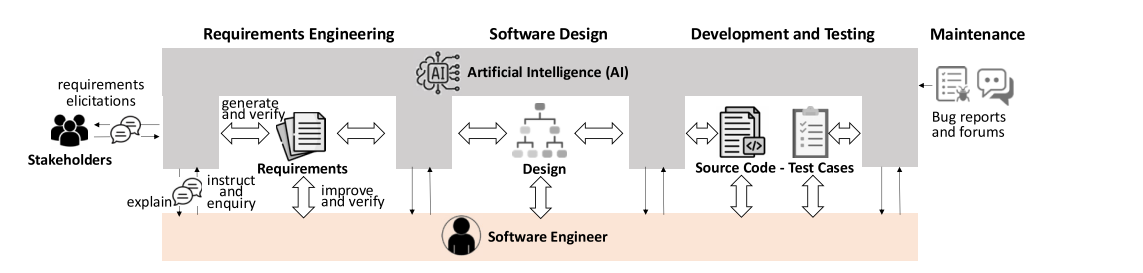
\includegraphics[width=\textwidth]{TESIS/CAPITULO-02/simbiosis_ia_se.png}
    \caption{Arquitectura lógica de la simbiosis futura entre ingenieros de software e IA\cite{Terragni2025}.}
    \label{fig:simbiosis_ia_se}
\end{figure}


La figura \ref{fig:simbiosis_ia_se} plantean una visión de simbiosis futura entre ingenieros de software e IA que abarca las principales 
fases del ciclo de vida del desarrollo: Ingeniería de Requisitos, Diseño de Software, Desarrollo y Pruebas, y Mantenimiento, tal como se ilustra 
en la Figura~\ref{fig:simbiosis_ia_se}. Según los autores, en la fase de requisitos los agentes de IA podrán asistir en la elicitación mediante 
conversaciones con los interesados, resumir documentación extensa y traducirla en especificaciones formales a partir de necesidades expresadas 
en lenguaje natural. Esta visión respalda el enfoque de la presente investigación, la cual se centra específicamente en automatizar dicha fase 
mediante un sistema multi-agente basado en MCP.



\subsection{Modelos de Lenguaje de Gran Escala (LLMs)}

Los Modelos de Lenguaje de Gran Escala (Large Language Models, LLMs) son sistemas de inteligencia artificial entrenados sobre grandes volúmenes de 
datos textuales con el objetivo de comprender, generar y transformar lenguaje natural. Estos modelos se basan principalmente en la arquitectura 
Transformer, la cual emplea mecanismos de atención para capturar relaciones contextuales entre palabras y secuencias de texto, permitiendo 
realizar tareas como generación de contenido, resumen automático, clasificación de información, traducción y asistencia en el 
desarrollo de software \cite{zadenoori2025large}, \cite{hemmat2025research}.

\begin{figure}[H]
    \centering
    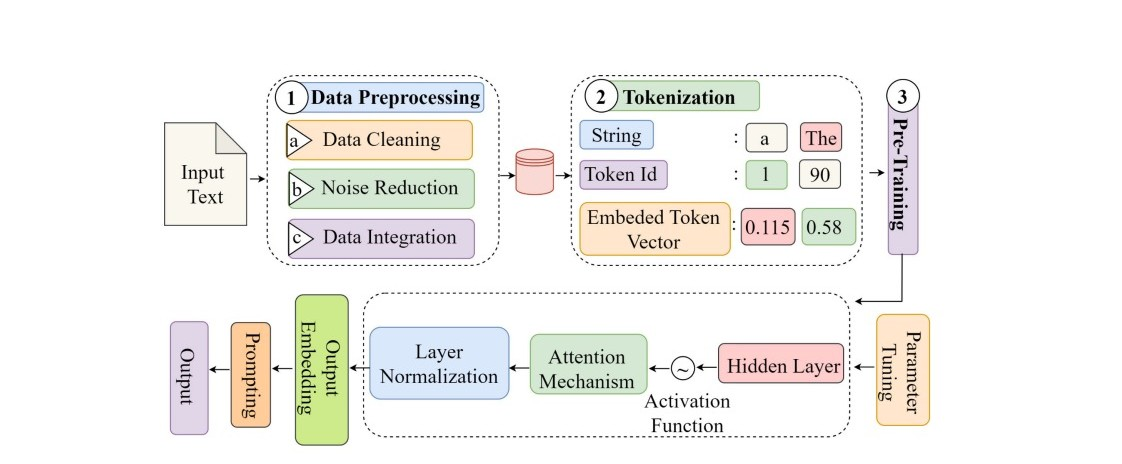
\includegraphics[width=\textwidth]{TESIS/CAPITULO-02/llm-pipeline.jpeg}
    \caption{Proceso general de funcionamiento de un LLM \cite{raiaan2024review}.}
    \label{fig:llm_pipeline}
\end{figure}

Raiaan et al. \cite{raiaan2024review} describen el proceso general de funcionamiento de un LLM como una secuencia de etapas que inicia con 
el preprocesamiento de los datos de entrada (limpieza, reducción de ruido e integración de datos), seguido de la tokenización, en la que el 
texto se convierte en identificadores numéricos y vectores de embedding. Posteriormente, durante la fase de preentrenamiento, el modelo ajusta 
sus parámetros mediante mecanismos de atención y normalización de capas, para finalmente generar una representación de salida 
(\textit{output embedding}) que es empleada en la etapa de \textit{prompting} para producir la respuesta final, tal como se ilustra en la 
Figura~\ref{fig:llm_pipeline}.



El desempeño de los LLMs ha impulsado su adopción en diferentes áreas de la Ingeniería de Software, incluyendo la Ingeniería de Requisitos, donde se 
utilizan para apoyar actividades de elicitación, análisis, validación y generación de especificaciones. Investigaciones recientes evidencian que estos 
modelos pueden contribuir a mejorar la calidad de documentos de requisitos, identificar inconsistencias y automatizar tareas tradicionalmente realizadas
por expertos humanos. Sin embargo, la mayoría de aplicaciones reportadas se desarrollan en entornos controlados y aún presentan limitaciones 
relacionadas con la precisión de las respuestas y la comprensión del contexto específico del dominio \cite{Umar2024}, \cite{khan2025large}.

Los LLMs constituyen el núcleo de procesamiento de los agentes inteligentes encargados de analizar transcripciones 
de entrevistas, clasificar requisitos funcionales y generar documentos de SRS conforme al estándar IEEE 830-1998. 
Su capacidad para interpretar lenguaje natural y producir texto estructurado permite automatizar actividades de Ingeniería de Requisitos que 
tradicionalmente requieren una elevada intervención manual \cite{Umar2024}, \cite{ellsel2025advancing}.


\subsection{Limitaciones de los LLMs}
A pesar de sus capacidades para comprender y generar texto en lenguaje natural, los Modelos de LLMs presentan diversas 
limitaciones que restringen su aplicación en dominios que requieren alta precisión, como la Ingeniería de Requisitos. Una de las principales 
problemáticas es la generación de información incorrecta o inexistente, fenómeno conocido como hallucination o alucinación, en el que el modelo 
produce respuestas plausibles pero sin sustento en fuentes verificables. Asimismo, estos modelos pueden heredar sesgos presentes en los datos de 
entrenamiento, afectando la objetividad y confiabilidad de los resultados generados \cite{ji2023survey}, \cite{rawte2023survey}.

Otra limitación importante corresponde a la gestión de contextos extensos y especializados. Aunque los LLMs modernos permiten procesar grandes 
cantidades de información, su desempeño puede degradarse cuando deben analizar documentos largos, múltiples conversaciones o información altamente 
específica de un dominio determinado. Adicionalmente, el conocimiento incorporado en el modelo se encuentra limitado a la fecha de corte de sus datos 
de entrenamiento, impidiendo acceder a información actualizada o a fuentes externas en tiempo real \cite{Guo2024}, \cite{hemmat2025research}.

Estas limitaciones resultan especialmente relevantes en tareas de Ingeniería de Requisitos, donde es necesario preservar la consistencia, completitud y 
trazabilidad de las especificaciones generadas. Por esta razón, investigaciones recientes han propuesto complementar los LLMs mediante técnicas de 
recuperación de información, arquitecturas multi-agente y mecanismos de inyección de contexto externo, con el propósito de mejorar la calidad de las 
respuestas y reducir la probabilidad de generar información errónea. En este trabajo de investigación, dichas limitaciones motivan la incorporación 
de un agente de enriquecimiento contextual y el uso del Model Context Protocol (MCP) para proporcionar información adicional a los modelos de lenguaje 
empleados \cite{Wolf2026}, \cite{Umar2024}.

\subsection{Retrieval-Augmented Generation (RAG)}

Retrieval-Augmented Generation (RAG) es una técnica que combina modelos de lenguaje de gran escala con mecanismos de recuperación de información 
externa para mejorar la precisión y actualidad de las respuestas generadas. A diferencia de los LLMs convencionales, que dependen únicamente del 
conocimiento adquirido durante su entrenamiento, RAG incorpora información relevante obtenida dinámicamente desde bases de datos, repositorios 
documentales o fuentes externas, permitiendo proporcionar respuestas fundamentadas en evidencia y reduciendo la probabilidad de generar información 
incorrecta o desactualizada \cite{gao2023retrieval}, \cite{lewis2020retrieval}.

El funcionamiento de RAG se basa generalmente en dos etapas principales: recuperación y generación. En la primera etapa, un sistema de búsqueda 
identifica y selecciona documentos o fragmentos de texto relacionados con la consulta del usuario mediante técnicas de similitud semántica o búsqueda 
vectorial. Posteriormente, la información recuperada es incorporada al contexto de entrada del modelo de lenguaje, el cual utiliza dichos datos para 
generar una respuesta más precisa y contextualizada. Este enfoque ha demostrado mejoras significativas en tareas de respuesta a preguntas, resumen 
automático, generación de código y aplicaciones especializadas en dominios como la medicina, 
educación e ingeniería de software \cite{gao2023retrieval}, \cite{huang2026survey}.

En el ámbito de la Ingeniería de Requisitos, RAG puede emplearse para enriquecer especificaciones obtenidas durante entrevistas de elicitación, 
proporcionando información complementaria proveniente de estándares, documentación técnica o fuentes de conocimiento especializadas. En esta 
investigación, el Agente de Enriquecimiento Contextual implementa un enfoque basado en RAG para complementar los requisitos funcionales identificados 
a partir de las transcripciones de entrevistas, utilizando información obtenida mediante servicios externos accesibles a través del MCP, con el propósito de 
mejorar la completitud y coherencia del documento SRS generado automáticamente \cite{lewis2020retrieval}, \cite{hemmat2025research}.



\section{Sistemas Multi-agente }

Los sistemas multiagente (MAS) son plataformas distribuidas compuestas por varios agentes autónomos que se comunican entre ellos y con el 
ambiente que los rodea, con el fin de dar solución a problemas complejos de forma colaborativa. Al repartir las tareas entre agentes con 
funciones específicas, se facilita el manejo de problemas que serían complejos de resolver con un solo elemento inteligente, lo que incrementa 
la capacidad de crecimiento, la adaptabilidad y la solidez del sistema.


\subsection{Definición y características de los agentes de IA}
Un agente de inteligencia artificial es una entidad de software capaz de percibir información de su entorno, procesarla, tomar decisiones 
y ejecutar acciones con el propósito de alcanzar objetivos específicos. A diferencia de los programas tradicionales, los agentes poseen 
cierto grado de autonomía y pueden adaptarse dinámicamente a cambios en el entorno, utilizando mecanismos de razonamiento, memoria y 
aprendizaje para mejorar su desempeño \cite{Guo2024}, \cite{zhang2025survey}.

Entre las principales características de los agentes de IA se encuentran la autonomía, que les permite operar sin intervención humana constante; 
la reactividad, que facilita responder a eventos del entorno; la proactividad, relacionada con la capacidad de anticiparse a situaciones futuras; y l
a habilidad social, que posibilita la interacción y cooperación con otros agentes o usuarios. En sistemas basados en LLMs, estas capacidades pueden 
complementarse mediante el uso de herramientas externas, memoria persistente y acceso a fuentes de conocimiento especializadas \cite{zhang2025survey}, \cite{durante2024agent}.

En esta investigación, cada agente especializado desempeña una función específica dentro del proceso de generación automática de documentos SRS. 
El agente de transcripción convierte el audio en texto, el agente de análisis identifica y clasifica requisitos funcionales, el agente de enriquecimiento
contextual recupera información adicional mediante RAG y el agente generador construye el documento SRS conforme al estándar IEEE 830-1998. 
La especialización de tareas permite reducir la complejidad del sistema y mejorar la calidad de los resultados obtenidos \cite{Guo2024}, \cite{xi2025rise}.


\subsection{Arquitecturas multi-agente basadas en LLMs}

Las arquitecturas multi-agente basadas en Modelos de Lenguaje de Gran Escala están compuestas por múltiples agentes inteligentes que colaboran 
para resolver tareas complejas mediante la distribución de responsabilidades y el intercambio de información. Cada agente puede estar especializado 
en actividades específicas, tales como planificación, razonamiento, recuperación de conocimiento, uso de herramientas externas o generación de 
contenido, permitiendo superar las limitaciones de los LLMs individuales \cite{Guo2024}, \cite{xi2025rise}.

Diversos estudios han propuesto arquitecturas organizadas de forma jerárquica, colaborativa o basada en roles. En las arquitecturas jerárquicas, 
un agente coordinador supervisa la ejecución de agentes subordinados, mientras que en las arquitecturas colaborativas los agentes intercambian 
información de manera descentralizada para alcanzar un objetivo común. También existen enfoques basados en roles, donde cada agente posee 
responsabilidades claramente definidas dentro del flujo de trabajo del sistema \cite{Guo2024}, \cite{durante2024agent}.


\begin{figure}[H]
    \centering
    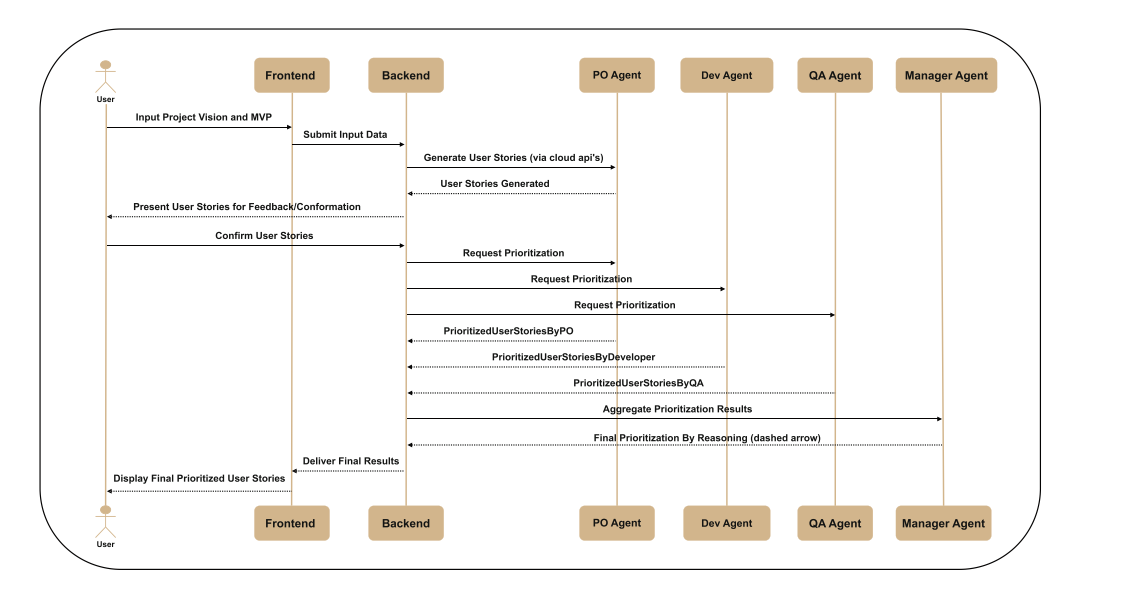
\includegraphics[width=\textwidth]{TESIS/CAPITULO-02/Sistema-multi-agente.png}
    \caption{Ejemplo de arquitectura multi-agente basada en roles para generación y priorización de historias de usuario \cite{Sami2026}.}
    \label{fig:arquitectura_roles}
\end{figure}



La Figura \ref{fig:arquitectura_roles} ilustra un ejemplo de arquitectura multi-agente basada en roles, en la que agentes especializados 
(Product Owner, Desarrollador, QA y Gestor) colaboran para generar y priorizar historias de usuario a partir de la visión del proyecto 
proporcionada por el usuario. En este esquema, un agente Manager centraliza las priorizaciones individuales emitidas por cada agente 
especializado y determina, mediante razonamiento, la priorización final que se entrega al usuario. Este tipo de coordinación evidencia 
cómo la especialización de roles y la comunicación estructurada entre agentes permiten resolver tareas colaborativas que un único modelo 
de lenguaje no podría abordar de forma aislada \cite{Sami2026}.




\subsection{Coordinación y comunicación entre agentes}

La coordinación y comunicación entre agentes constituyen elementos fundamentales en los sistemas multi-agente, ya que permiten organizar 
la ejecución de tareas, intercambiar información y alcanzar objetivos comunes de manera eficiente. En arquitecturas basadas en inteligencia 
artificial generativa, la coordinación puede realizarse mediante agentes supervisores u orquestadores encargados de asignar responsabilidades, 
controlar el flujo de trabajo y gestionar la interacción entre agentes especializados. Este enfoque contribuye a mejorar la modularidad, 
escalabilidad y capacidad de adaptación del sistema ante cambios en los requerimientos o en el entorno de operación \cite{Guo2024}, \cite{xi2025rise}.

Los mecanismos de comunicación entre agentes pueden implementarse utilizando intercambio de mensajes, memoria compartida, bases de conocimiento 
comunes o protocolos estandarizados que faciliten la interoperabilidad entre componentes heterogéneos. En sistemas multi-agente basados en LLMs, 
la comunicación estructurada permite transmitir instrucciones, resultados parciales y contexto adicional entre agentes, reduciendo la pérdida de 
información y favoreciendo procesos colaborativos de razonamiento. Asimismo, la incorporación de herramientas externas y servicios especializados 
amplía las capacidades de los agentes, permitiéndoles acceder a información actualizada y ejecutar acciones fuera de las capacidades intrínsecas 
del modelo de lenguaje \cite{Guo2024}, \cite{durante2024agent}.

En esta investigación, la coordinación del sistema es realizada por un Agente Orquestador que dirige la ejecución secuencial de los agentes de 
transcripción, análisis y clasificación, enriquecimiento contextual y generación del documento SRS. La comunicación entre estos agentes y los 
servicios externos se gestiona mediante el MCP, el cual proporciona una interfaz estandarizada para intercambiar contexto, 
invocar herramientas y acceder a recursos externos, garantizando un flujo de información estructurado durante el proceso de generación automatizada 
del documento de especificación de requisitos \cite{xi2025rise}, \cite{zhang2025survey}.

\subsection{Frameworks para sistemas multi-agente}

Los frameworks para sistemas multi-agente proporcionan componentes reutilizables y mecanismos de abstracción que facilitan el desarrollo, 
coordinación y ejecución de agentes inteligentes. En el contexto de aplicaciones basadas en Modelos de Lenguaje de Gran Escala (LLMs), estos 
frameworks permiten definir roles especializados, administrar estados conversacionales, integrar herramientas externas y gestionar flujos de 
trabajo complejos, reduciendo el esfuerzo de implementación y mejorando la mantenibilidad de las soluciones desarrolladas \cite{Guo2024}, \cite{xi2025rise}.

Entre los frameworks más utilizados se encuentran AutoGen, LangGraph, CrewAI y Semantic Kernel. AutoGen permite construir conversaciones 
entre múltiples agentes autónomos capaces de colaborar para resolver tareas complejas, mientras que LangGraph facilita la definición de 
flujos de trabajo mediante grafos dirigidos y estados persistentes. Por su parte, CrewAI se orienta a la creación de equipos de agentes 
con roles específicos y Semantic Kernel proporciona mecanismos para integrar modelos de lenguaje con herramientas, memoria y servicios 
externos \cite{xi2025rise}, \cite{wu2023autogen}. Estas plataformas han ganado relevancia debido a su flexibilidad para implementar arquitecturas multi-agente en aplicaciones 
de automatización, asistencia inteligente e ingeniería de software.

En esta investigación, aunque el sistema propuesto no depende de un framework multi-agente específico, las capacidades ofrecidas por estas 
herramientas constituyen una referencia para el diseño de la arquitectura planteada. En particular, la existencia de un agente orquestador, 
agentes especializados y mecanismos de comunicación con servicios externos guarda similitud con las estrategias de coordinación implementadas 
en dichos frameworks, facilitando además una posible evolución futura del prototipo hacia soluciones más robustas y escalables \cite{Guo2024}.



\section{Model Context Protocol (MCP) }

El Protocolo de Contexto para Modelos (MCP, por sus siglas en inglés) se presenta como un estándar pensado para simplificar la comunicación entre 
modelos de lenguaje de gran escala y elementos externos, brindando un acceso ordenado a herramientas, bases de datos y servicios especializados. 
Su finalidad fundamental es potenciar las habilidades de los sistemas de inteligencia artificial al integrar información contextual en tiempo real 
y facilitar la conexión entre distintas aplicaciones.\cite{Anthropic2024}

\subsection{Definición y propósito del MCP}

El MCP es un estándar abierto que define una forma uniforme de vincular modelos lingüísticos con herramientas, 
repositorios de datos y servicios externos. Su meta es brindar a los sistemas de inteligencia artificial un acceso regulado a información 
complementaria y a funciones que van más allá de su conocimiento base, lo que les permite potenciar su capacidad de razonamiento y la ejecución 
de tareas complejas. Con ello, el protocolo pretende dar respuesta a inconvenientes como la carencia de datos recientes, la excesiva dependencia 
del conjunto de entrenamiento y las complicaciones para articular diversos servicios en una sola plataforma.

La arquitectura propuesta integra el MCP para operacionalizar un enfoque inspirado en arquitecturas orientadas a servicios, 
bajo el cual los agentes inteligentes pueden solicitar información o ejecutar acciones a través de servidores especializados que exponen recursos y 
herramientas específicas. Esta estrategia técnica se fundamenta en la capacidad de uso de herramientas (tool-use), la cual permite a los modelos de 
lenguaje aprovechar recursos externos para ampliar sus funciones y operar de manera más efectiva en entornos diversos . Este diseño modular favorece 
la interoperabilidad entre aplicaciones heterogéneas y maximiza la reutilización de componentes, permitiendo incorporar nuevas capacidades al sistema 
sin necesidad de modificar o reentrenar el modelo de lenguaje subyacente \cite{Guo2024}

En esta investigación, se implementa el MCP como el mecanismo de comunicación para conectar los agentes especializados 
con servicios externos de búsqueda web, almacenamiento de documentos y generación del documento SRS. Su utilización permite operacionalizar la 
inyección de contexto adicional a los agentes inteligentes, mejorando la calidad de la información procesada y mitigando el riesgo de alucinaciones.
Asimismo, este enfoque garantiza una arquitectura modular que facilita la gestión del sistema y futuras ampliaciones del prototipo desarrollado
\cite{Guo2024}, \cite{xi2025rise}.

\subsection{Arquitectura cliente-servidor}
El MCP se basa en un modelo arquitectónico cliente-servidor que posibilita una interacción estandarizada entre 
aplicaciones impulsadas por modelos de lenguaje y servicios externos. Bajo este enfoque, el cliente MCP se encarga de originar las peticiones 
y de coordinar la comunicación con uno o múltiples servidores MCP, mientras que estos últimos ponen a disposición recursos, herramientas y 
capacidades que el modelo de lenguaje puede aprovechar al momento de ejecutar una tarea concreta.Esta separación de responsabilidades facilita la 
modularidad del sistema y permite incorporar nuevas capacidades sin modificar la lógica interna del modelo de inteligencia artificial.

La arquitectura propuesta utiliza el MCP como mecanismo para establecer una comunicación estructurada entre clientes y 
servidores mediante el intercambio de mensajes en formatos estandarizados. Su implementación permite descubrir capacidades disponibles en servidores 
especializados y conectar a un mismo cliente con múltiples fuentes de información, tales como motores de búsqueda, bases de datos o sistemas de archivos. 
Esta estrategia técnica se fundamenta en la capacidad de uso de herramientas (tool-use), la cual favorece la interoperabilidad entre componentes 
heterogéneos y simplifica la integración de recursos externos dentro de aplicaciones basadas en Modelos de Lenguaje de Gran Escala \cite{Guo2024}.

En la presente investigación, el Agente Orquestador desempeña el rol de cliente MCP, coordinando la comunicación con diversos servidores especializados. 
Entre ellos se encuentran un servidor de búsqueda web para el enriquecimiento contextual de requisitos, un servidor de base de datos encargado del 
almacenamiento de documentos SRS generados y un servidor orientado al soporte de generación estructurada del documento final. Esta arquitectura 
permite desacoplar los servicios externos de los procesos cognitivos de los agentes, siguiendo los principios de modularidad y orquestación 
propuestos por \cite{Guo2024},lo que facilita la escalabilidad y especialización necesaria para tareas de ingeniería de requisitos complejas \cite{xi2025rise}.

\subsection{Resources, Tools y Prompts}

Los conceptos de Resources, Tools y Prompts constituyen los elementos fundamentales del MCP, permitiendo estandarizar la 
interacción entre modelos de lenguaje y servicios externos. Los Resources representan fuentes de información que pueden ser consultadas por un modelo,
tales como documentos, archivos, bases de datos o contenido web. Los Tools corresponden a funciones ejecutables expuestas por un servidor MCP que 
permiten al modelo interactuar con el entorno mediante acciones que generan efectos secundarios, tales como efectuar búsquedas, consultar repositorios, 
modificar bases de datos o invocar APIs externas. Finalmente, los Prompts actúan como plantillas reutilizables que estructuran la interacción, 
permitiendo una orquestación de flujos de trabajo más eficiente \cite{hou2025model}.

\begin{figure}[H]
    \centering
    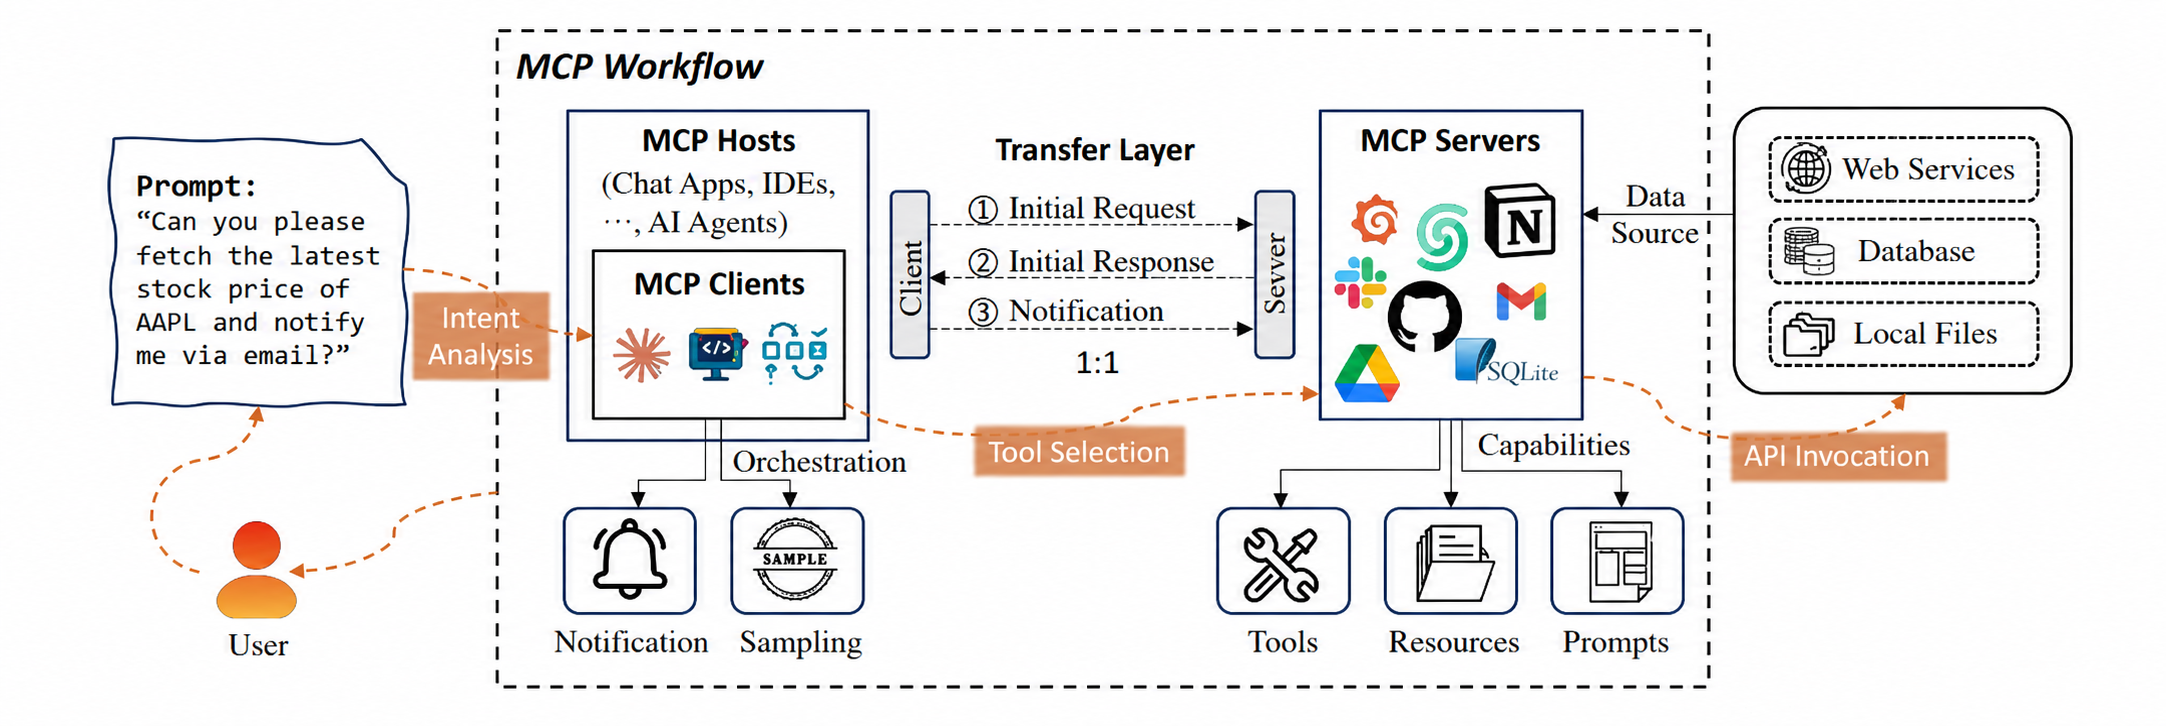
\includegraphics[width=\textwidth]{TESIS/CAPITULO-02/mcp-workflow.png}
    \caption{Flujo de trabajo del Model Context Protocol \cite{hou2025model}.}
    \label{fig:mcp_workflow}
\end{figure}

La Figura~\ref{fig:mcp_workflow} ilustra el flujo de trabajo completo del MCP, desde que el usuario formula una solicitud en lenguaje natural hasta 
la ejecución de las capacidades correspondientes. El MCP Host aloja al cliente MCP, el cual envía una solicitud inicial al servidor a través de la 
capa de transferencia, estableciendo una comunicación de tipo 1:1 entre cliente y servidor. Una vez seleccionada la herramienta apropiada mediante el 
proceso de \textit{Tool Selection}, el servidor expone sus capacidades organizadas en las tres categorías mencionadas: Tools, Resources y Prompts, 
las cuales son invocadas para satisfacer la intención detectada en la solicitud del usuario \cite{hou2025model}.

La separación entre recursos, herramientas y prompts permite desacoplar el contexto informativo, las capacidades operativas y las estructuras de 
interacción de un sistema basado en LLMs. Esta organización favorece el descubrimiento dinámico de capacidades en servidores MCP y mejora la 
interoperabilidad en entornos heterogéneos. Investigaciones recientes como ScaleMCP demuestran que esta arquitectura, combinada con mecanismos de 
auto-sincronización, permite a los agentes gestionar de forma autónoma un vasto ecosistema de herramientas, superando las limitaciones de conocimiento 
estático y proporcionando acceso a datos en tiempo real fuera del alcance interno del modelo \cite{hou2025model}, \cite{lumer2025scalemcp}.

En el contexto del presente trabajo, los servidores MCP implementados exponen principalmente herramientas (Tools) para la búsqueda de información y 
almacenamiento de documentos, mientras que los Prompts son utilizados internamente por los agentes para estructurar la generación del documento SRS.

\subsection{Integración del MCP con agentes de IA}

La integración del MCP con agentes de inteligencia artificial permite ampliar las capacidades de los modelos de 
lenguaje mediante el acceso estandarizado a recursos, herramientas y servicios externos. En lugar de depender únicamente del conocimiento adquirido 
durante el entrenamiento, los agentes pueden utilizar MCP para consultar información actualizada, ejecutar acciones específicas y compartir contexto 
con otros componentes del sistema. Este enfoque favorece el desarrollo de agentes más autónomos, adaptables y capaces de resolver tareas complejas que 
requieren interacción con múltiples fuentes de información \cite{hou2025model}.

En arquitecturas multi-agente basadas en LLMs, MCP actúa como una capa de interoperabilidad que facilita la comunicación entre agentes 
especializados y servidores externos. A través de este protocolo, los agentes pueden descubrir dinámicamente las capacidades disponibles, 
invocar herramientas remotas y acceder a recursos compartidos sin necesidad de implementar integraciones específicas para cada servicio. 
Investigaciones recientes destacan que esta capacidad contribuye a mejorar la modularidad, escalabilidad y mantenibilidad de sistemas inteligentes 
compuestos por múltiples agentes colaborativos \cite{hou2025model}, \cite{lumer2025scalemcp}.

En la presente investigación, el Agente Orquestador desempeña el rol de cliente MCP, coordinando la comunicación con diversos servidores 
especializados bajo el estándar abierto introducido por \cite{Anthropic2024}. Entre estos servidores se incluyen uno de búsqueda web para el 
enriquecimiento contextual de requisitos, uno de base de datos para el almacenamiento de documentos SRS y un servidor orientado al soporte de 
generación estructurada. Esta arquitectura permite desacoplar los servicios externos de los procesos cognitivos de los agentes, facilitando la 
escalabilidad y el mantenimiento del sistema multi-agente propuesto, en línea con los principios de orquestación y especialización requeridos para 
tareas de ingeniería de requisitos de alta complejidad \cite{Guo2024}, \cite{xi2025rise}.





\section{Reconocimiento Automático de Voz (ASR) }

El Reconocimiento Automático de Voz (Automatic Speech Recognition, ASR) es una tecnología de inteligencia artificial que permite convertir 
señales de audio habladas en texto legible por máquinas. Gracias a los avances recientes en aprendizaje profundo y modelos neuronales de gran 
escala, los sistemas ASR han alcanzado niveles de precisión que posibilitan su aplicación en diversos dominios, incluyendo asistentes virtuales, 
sistemas de transcripción, atención al cliente e Ingeniería de Software \cite{Li2020}, \cite{Radford2022}

En el contexto de la Ingeniería de Requisitos, el ASR representa una alternativa prometedora para automatizar la transcripción de entrevistas de 
elicitación, reduciendo el esfuerzo manual asociado a la documentación y facilitando el procesamiento posterior de la información mediante modelos 
de lenguaje y sistemas multi-agente \cite{Radford2022}, \cite{Umar2024}.

\subsection{Fundamentos del ASR}

El Reconocimiento Automático de Voz (Automatic Speech Recognition, ASR) es una tecnología que permite transformar señales de voz en texto mediante 
técnicas de procesamiento digital de señales y aprendizaje automático. Los sistemas ASR modernos emplean modelos neuronales profundos capaces de 
aprender representaciones acústicas y lingüísticas directamente a partir de grandes volúmenes de datos, eliminando la necesidad de diseñar manualmente 
características específicas del habla. El objetivo principal de estos sistemas es minimizar la tasa de error de palabras (Word Error Rate, WER) y generar 
transcripciones precisas incluso en presencia de ruido, variaciones de pronunciación o diferencias entre hablantes \cite{Radford2022}.

El proceso de reconocimiento de voz comprende generalmente varias etapas, incluyendo el preprocesamiento de la señal de audio, la extracción de 
características acústicas, el modelado acústico, el modelado del lenguaje y la decodificación de la secuencia de palabras más probable. En los últimos 
años, las arquitecturas basadas en Transformers y modelos de aprendizaje autosupervisado han demostrado mejoras significativas respecto a enfoques 
tradicionales basados en modelos ocultos de Markov y redes neuronales recurrentes, permitiendo obtener sistemas más robustos y capaces de generalizar a 
diferentes idiomas y dominios de aplicación \cite{baevski2020wav2vec}.

En el contexto de esta investigación, el ASR constituye el primer componente del sistema multi-agente propuesto, siendo responsable de convertir los 
audios de entrevistas realizadas a Product Owners en transcripciones textuales que posteriormente serán procesadas por agentes especializados en análisis, 
enriquecimiento contextual y generación automática del documento SRS. La precisión alcanzada durante esta etapa resulta fundamental, ya que errores en la 
transcripción pueden propagarse al resto del flujo de procesamiento y afectar la calidad de las especificaciones generadas \cite{Radford2022}, \cite{Umar2024}.



\subsection{Modelos open source para transcripción}

Los avances recientes en reconocimiento automático de voz han impulsado el desarrollo de diversos modelos de código abierto capaces de realizar 
transcripciones con altos niveles de precisión. Entre los más destacados se encuentra Whisper, desarrollado por OpenAI, el cual fue entrenado 
mediante aprendizaje débilmente supervisado utilizando aproximadamente 680 000 horas de datos de audio multilingües recopilados de Internet. 
Gracias a esta estrategia, Whisper presenta una elevada robustez frente a ruido de fondo, acentos y variaciones lingüísticas. Esto le permite 
generalizar con éxito en un entorno zero-shot, logrando resultados competitivos en diversos dominios sin necesidad de un ajuste fino (fine-tuning) 
específico para cada conjunto de datos \cite{Radford2022}.

Otro modelo ampliamente utilizado es wav2vec 2.0, propuesto por Meta AI, que emplea aprendizaje autosupervisado para obtener representaciones del habla 
a partir de grandes cantidades de audio sin etiquetar \cite{baevski2020wav2vec}. Tras un proceso de ajuste fino con datos anotados, este modelo logra 
desempeños competitivos en diferentes conjuntos de evaluación, destacando por su eficiencia en entornos de bajos recursos de 
datos \cite{baevski2020wav2vec}, \cite{Radford2022}. Asimismo, DeepSpeech constituye una alternativa de código abierto basada en redes neuronales 
profundas, cuya arquitectura ha facilitado el despliegue de sistemas de reconocimiento de voz robustos en diversos dominios operativos \cite{Radford2022}.

El uso de modelos open source para transcripción resulta adecuado debido a su flexibilidad, disponibilidad y capacidad para 
integrarse dentro de arquitecturas multi-agente. Particularmente, Whisper representa una opción prometedora para el Agente de Transcripción ASR, ya 
que ofrece soporte multilingüe, alta precisión en escenarios reales y puede ejecutarse localmente o mediante servicios externos, facilitando su 
incorporación al prototipo propuesto para procesar entrevistas de elicitación. En este flujo, el ASR permite transformar el lenguaje natural de 
los interesados en datos procesables por el sistema multi-agente, optimizando la captura de necesidades técnicas \cite{Radford2022}, \cite{Akhtar2025}.

\subsection{ASR aplicado a entrevistas de elicitación }

Las entrevistas constituyen una de las técnicas de elicitación de requisitos más utilizadas en Ingeniería de Requisitos, ya que permiten obtener 
información detallada sobre las necesidades, expectativas y restricciones de los interesados. Sin embargo, la documentación manual de estas sesiones 
suele ser una actividad tediosa y propensa a errores, especialmente cuando las entrevistas poseen una larga duración o involucran múltiples 
participantes. En este contexto, los sistemas de Reconocimiento Automático de Voz (ASR) ofrecen una alternativa para automatizar la transcripción de 
las conversaciones, facilitando su posterior análisis y procesamiento \cite{Radford2022}, \cite{Umar2024}.

La incorporación de tecnologías ASR en procesos de elicitación permite disponer de registros textuales completos de las entrevistas, reduciendo la 
pérdida de información y mejorando la trazabilidad entre las necesidades expresadas por los usuarios y los requisitos documentados. Asimismo, las 
transcripciones generadas pueden ser procesadas mediante modelos de lenguaje de gran escala para identificar requisitos funcionales, detectar 
inconsistencias y asistir en la construcción de documentos de especificación. Estudios recientes evidencian un creciente interés por combinar 
técnicas de procesamiento del lenguaje natural e inteligencia artificial para brindar soporte automatizado a actividades de Ingeniería 
de Requisitos \cite{Umar2024}, \cite{Wolf2026}.

El ASR representa el punto de partida del flujo de procesamiento del sistema multi-agente propuesto. El agente de 
transcripción recibe el audio de entrevistas realizadas a Product Owners y genera una representación textual que posteriormente es utilizada por 
agentes especializados en análisis, enriquecimiento contextual y generación del documento SRS conforme al estándar IEEE 830-1998. De esta manera, 
la automatización de la transcripción contribuye a disminuir el esfuerzo asociado a la documentación manual y proporciona una base estructurada 
para las etapas posteriores del proceso \cite{Radford2022}, \cite{Wolf2026}.



\subsection{Integración del ASR en sistemas multi-agente}

La integración del Reconocimiento Automático de Voz (ASR) en sistemas multi-agente permite distribuir las tareas de procesamiento del habla y 
análisis de información entre componentes especializados, mejorando la modularidad y escalabilidad de la solución desarrollada. En este enfoque, 
un agente dedicado al reconocimiento de voz es responsable de transformar el audio en texto, mientras que otros agentes pueden encargarse del 
análisis semántico, recuperación de información, razonamiento o generación de documentos. Esta separación de responsabilidades facilita el mantenimiento 
del sistema y permite sustituir o actualizar componentes individuales sin afectar el funcionamiento global de la 
arquitectura \cite{Radford2022}, \cite{Guo2024}.


Las arquitecturas multi-agente basadas en modelos de lenguaje han demostrado ser adecuadas para resolver tareas complejas que requieren el 
procesamiento secuencial de información proveniente de distintas fuentes. La incorporación de un agente ASR como etapa inicial del flujo de 
trabajo posibilita capturar conocimiento expresado verbalmente y convertirlo en información estructurada que puede ser utilizada por otros agentes 
especializados. Además, la combinación de tecnologías ASR con modelos de lenguaje de gran escala favorece la automatización de procesos que 
tradicionalmente dependen de intervención humana, incluyendo actividades relacionadas con la Ingeniería de Requisitos \cite{Guo2024}, \cite{Umar2024}.

En la presente investigación, el Agente de Transcripción ASR constituye el primer componente del sistema multi-agente propuesto y tiene la 
responsabilidad de procesar los audios de entrevistas realizadas a Product Owners. La salida generada por este agente es enviada al Agente 
de Análisis y Clasificación, encargado de identificar requisitos funcionales, para posteriormente ser enriquecida mediante técnicas RAG y utilizada 
en la construcción automática del documento SRS conforme al estándar IEEE 830-1998. Esta integración permite establecer un flujo de procesamiento 
organizado y favorece la generación de especificaciones de requisitos con menor intervención manual \cite{Radford2022}, \cite{Wolf2026}.



\section{Arquitectura e Integración de Aplicaciones Web}

El desarrollo de aplicaciones web ha evolucionado significativamente con la adopción de arquitecturas desacopladas y servicios distribuidos, 
permitiendo construir sistemas más escalables, mantenibles y adaptables a diferentes entornos de ejecución. Estas aplicaciones suelen estar 
compuestas por componentes especializados que interactúan a través de interfaces bien definidas, facilitando la integración de tecnologías 
emergentes como modelos de lenguaje, sistemas multi-agente y servicios de inteligencia artificial \cite{richards2020fundamentals}, \cite{newman2021building}.

En el marco de este estudio, la plataforma web actúa como el canal de comunicación entre el usuario y el sistema multi-agente diseñado, 
facilitando la carga de grabaciones de entrevistas para la obtención de requisitos, la consulta de los documentos SRS generados y el resguardo 
de los datos obtenidos. En los apartados siguientes se detallan los fundamentos de las arquitecturas web, las formas de conexión entre el frontend, 
el backend y los agentes inteligentes, así como las técnicas empleadas para mostrar los resultados y los informes generados.



\subsection{Arquitectura de aplicaciones web}

Las arquitecturas de aplicaciones web definen la organización de los componentes de software y las interacciones necesarias para proporcionar 
servicios a los usuarios finales. Tradicionalmente, estas arquitecturas se estructuran en capas diferenciadas, donde el frontend se encarga de 
la interfaz de usuario, el backend procesa la lógica de negocio y las bases de datos gestionan la persistencia de la información. Esta separación 
favorece la mantenibilidad, reutilización de componentes y escalabilidad de la aplicación \cite{richards2020fundamentals}, \cite{newman2021building}.

En aplicaciones modernas, es común adoptar arquitecturas basadas en APIs REST, las cuales permiten establecer mecanismos de comunicación independientes 
de la tecnología utilizada en cada componente. De esta manera, clientes web, servicios de inteligencia artificial y sistemas externos pueden 
intercambiar información mediante solicitudes HTTP estandarizadas, facilitando la integración de funcionalidades distribuidas. No obstante, 
esta estructura requiere una gestión rigurosa de la latencia de red y la implementación de controles de seguridad en cada punto de conexión, 
dado que la superficie de ataque aumenta en comparación con las arquitecturas monolíticas \cite{newman2021building}, \cite{richards2020fundamentals}.

En este trabajo, la aplicación web se desarrolló bajo un esquema arquitectónico de capas múltiples, en el que una interfaz gráfica posibilita 
la carga de archivos de audio provenientes de entrevistas y la revisión de los documentos SRS producidos. El backend funciona como puente entre 
el usuario y el sistema multia-gente, encargándose de recibir peticiones, orquestar el flujo de procesamiento de los datos y conservar los resultados 
generados, de modo que puedan ser recuperados y analizados posteriormente.

\subsection{Integración entre frontend, backend y agentes}

La integración entre el frontend, el backend y los agentes inteligentes es un aspecto fundamental en aplicaciones basadas en arquitecturas 
distribuidas, ya que permite coordinar el intercambio de información entre la interfaz de usuario y los componentes encargados del procesamiento 
de datos. Generalmente, el frontend actúa como punto de interacción con el usuario, mientras que el backend implementa la lógica de negocio, 
expone servicios mediante APIs REST y gestiona la comunicación con otros módulos especializados \cite{richards2020fundamentals}, \cite{newman2021building}.

En sistemas multi-agente basados en modelos de lenguaje, el backend puede desempeñar el papel de intermediario entre la aplicación web y los 
agentes inteligentes, recibiendo solicitudes, orquestando la ejecución de tareas y consolidando los resultados obtenidos. Esta estrategia 
facilita la incorporación de agentes especializados para actividades como transcripción de audio, análisis de información, recuperación de 
contexto y generación de documentos, manteniendo desacoplados los componentes de presentación y procesamiento \cite{newman2021building}, \cite{Guo2024}.

En este estudio, la plataforma web ofrece al usuario la opción de subir grabaciones de entrevistas de elicitación y acceder a los documentos 
SRS generados de forma automatizada. Tras recibir el archivo de audio, el backend lo remite al Agente Orquestador, quien se encarga de dirigir 
la ejecución ordenada de los agentes especializados en transcripción ASR, análisis y categorización, enriquecimiento contextual y redacción del 
documento SRS. Por último, el informe resultante se guarda en la base de datos y se muestra al usuario en la interfaz web, permitiendo su revisión 
y comparación en etapas posteriores.



\subsection{Visualización de resultados y reportes}
La visualización de resultados constituye un componente esencial en aplicaciones web modernas, ya que permite presentar información procesada 
de forma clara, organizada y comprensible para los usuarios. Una adecuada representación de los datos facilita la interpretación de los resultados 
obtenidos, mejora la experiencia de uso del sistema y contribuye a la toma de decisiones informadas. En aplicaciones de apoyo a la Ingeniería de 
Software, la presentación estructurada de documentos, métricas y reportes favorece además las actividades de revisión, validación y comparación de 
artefactos generados automáticamente \cite{richards2020fundamentals}, \cite{newman2021building}.

Las aplicaciones web actuales suelen incorporar mecanismos de visualización dinámica que permiten mostrar documentos, tablas, indicadores y 
reportes generados por procesos automatizados. En sistemas basados en inteligencia artificial, estas interfaces posibilitan que los usuarios 
inspeccionen los resultados producidos por modelos de aprendizaje automático, realicen validaciones manuales y almacenen información para 
consultas posteriores. Asimismo, la persistencia de los resultados facilita mantener un historial de ejecuciones y efectuar análisis comparativos 
entre diferentes versiones o documentos generados \cite{richards2020fundamentals}, \cite{Umar2024}.

En el marco de esta investigación, la interfaz web exhibe el documento SRS producido automáticamente bajo los lineamientos del estándar 
IEEE 830-1998, ofreciendo al usuario una presentación ordenada de los requisitos funcionales extraídos durante la entrevista de elicitación. 
Asimismo, el sistema resguarda los informes generados en una base de datos, lo que facilita su recuperación, exportación y confrontación futura 
con especificaciones realizadas de forma manual, contribuyendo así al proceso de validación del prototipo desarrollado.